
\documentclass[11pt]{article}
\PassOptionsToPackage{svgnames}{xcolor}
\usepackage{graphicx} % Required for inserting images
\usepackage[utf8]{inputenc}
\usepackage[margin=1in]{geometry}
\usepackage{enumerate, fancyhdr, color, verbatim, setspace, multirow, multicol,subcaption, booktabs, caption, amsfonts}
\usepackage{rotating}
\usepackage{amsmath}
\usepackage{amsthm}
\usepackage{cancel}
\usepackage{listings}
\numberwithin{equation}{section}
\newtheorem{definition}{Definition}[subsection]
\newtheorem{theorem}{Theorem}[subsection]
\newtheorem{corollary}{Corollary}[subsection]
\newcommand{\E}{\mathbb{E}}
\newcommand{\Var}{\mathbb{V}}


\usepackage{colortbl}
\usepackage{tikz}
\usetikzlibrary{matrix, positioning, shadings, shadows}
\usepackage{pgfplots}
\pgfplotsset{compat=1.18}
\usepackage[shortlabels]{enumitem}
% \usepackage[symbol]{footmisc}
\usepackage{multirow}
\usepackage{multicol}
% Creates the header and footer. You can adjust the look and feel of these here.
\usepackage{hyperref}
\hypersetup{
    colorlinks,
    citecolor=black,
    filecolor=black,
    linkcolor=blue,
    urlcolor=blue
}
\newcommand{\bp}{\mathbb{P}}

\definecolor{lightgray}{RGB}{230, 230, 230}
\definecolor{lightgrey}{RGB}{200, 200, 200}

\usepackage{tcolorbox}
\newenvironment{myblock}[1]{%
    \tcolorbox[beamer,%
    noparskip,breakable,
    colback=lightgray,colframe=black,%
    colbacklower=lightgrey,%
    title=#1]}%
    {\endtcolorbox}

\tcbuselibrary{skins,breakable}


\renewcommand{\headrulewidth}{0.2pt} %Creates a horizontal line underneath the header
\setlength{\headheight}{15pt} %Sets enough space for the header
% \renewcommand{\theenumi}{\alph{enumi}}
\onehalfspacing

\usepackage{chngcntr}
\counterwithin{figure}{section}

\DeclareMathOperator*{\argmin}{arg\,min}
\DeclareMathOperator*{\argmax}{arg\,max}

\usepackage[backend=biber, style=authoryear, maxcitenames=2, maxbibnames=9]{biblatex}
\DeclareDelimFormat{nameyeardelim}{\addcomma\space}
\addbibresource{references.bib}

\setcounter{tocdepth}{2}

\title{MGTECON 603 - Problem Set 2\\ \small{(Instructor: Guido Imbens)}}
\author{Wooyong Park\\ {\small Collaborators: Cem Kozanoglu, Roberto Gonzalez Tellez, Hanniel Ho, Aileen Wu}}
\date{\today}

\begin{document}


\maketitle

\section{Part I}

\subsection*{Descriptive Statistics}

The summary statistics of the data are shown in tables \ref{tab:summary_stats}, \ref{tab:summary_stats(control_group)}, and \ref{tab:summary_stats(treated_group)} in the appendix.

The histogram of the outcome variable \verb|earnings1yr| (Figure \ref{fig:hist_earnings1yr}) displays a heavily zero-inflated distribution, and overall we have more treated units than control units.

\begin{figure}[h]
    \centering
    \begin{subfigure}{0.48\textwidth}
        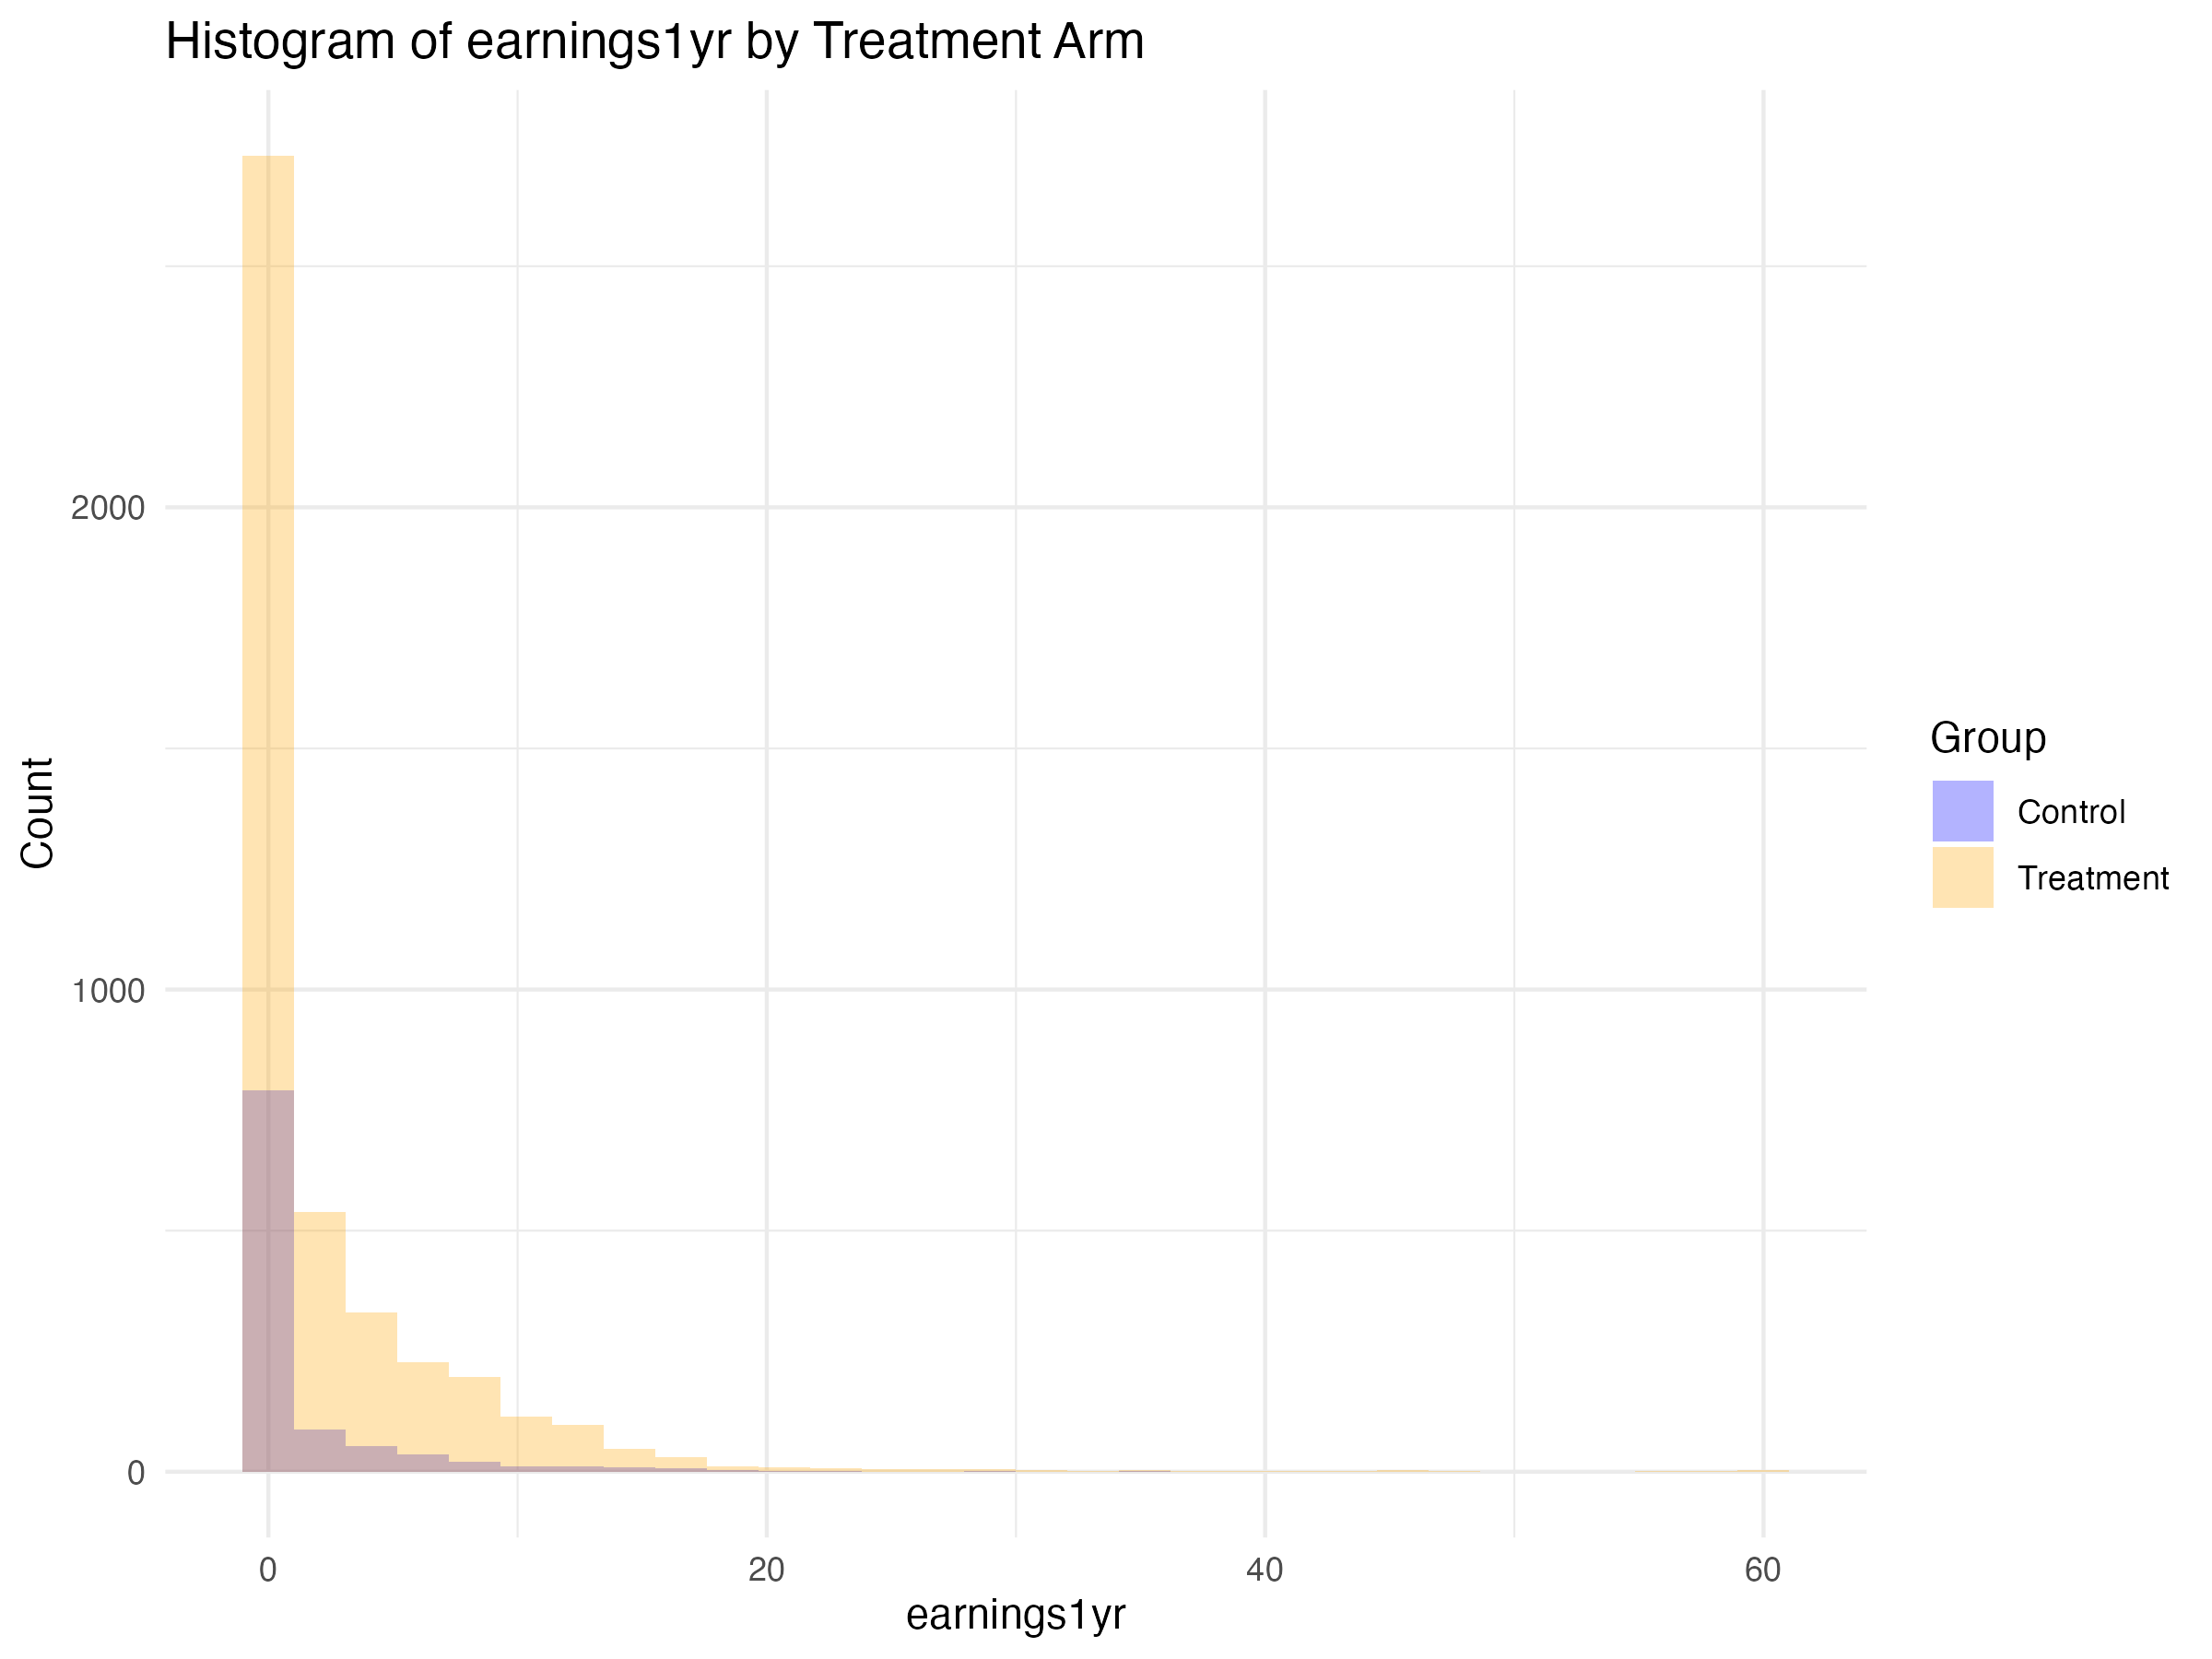
\includegraphics[width=0.8\textwidth]{output/histogram_earnings1yr_by_treatment_arm.png}
        \caption{\label{fig:hist_earnings1yr}Earnings one year after treatment}
    \end{subfigure}
    \begin{subfigure}{0.48\textwidth}
        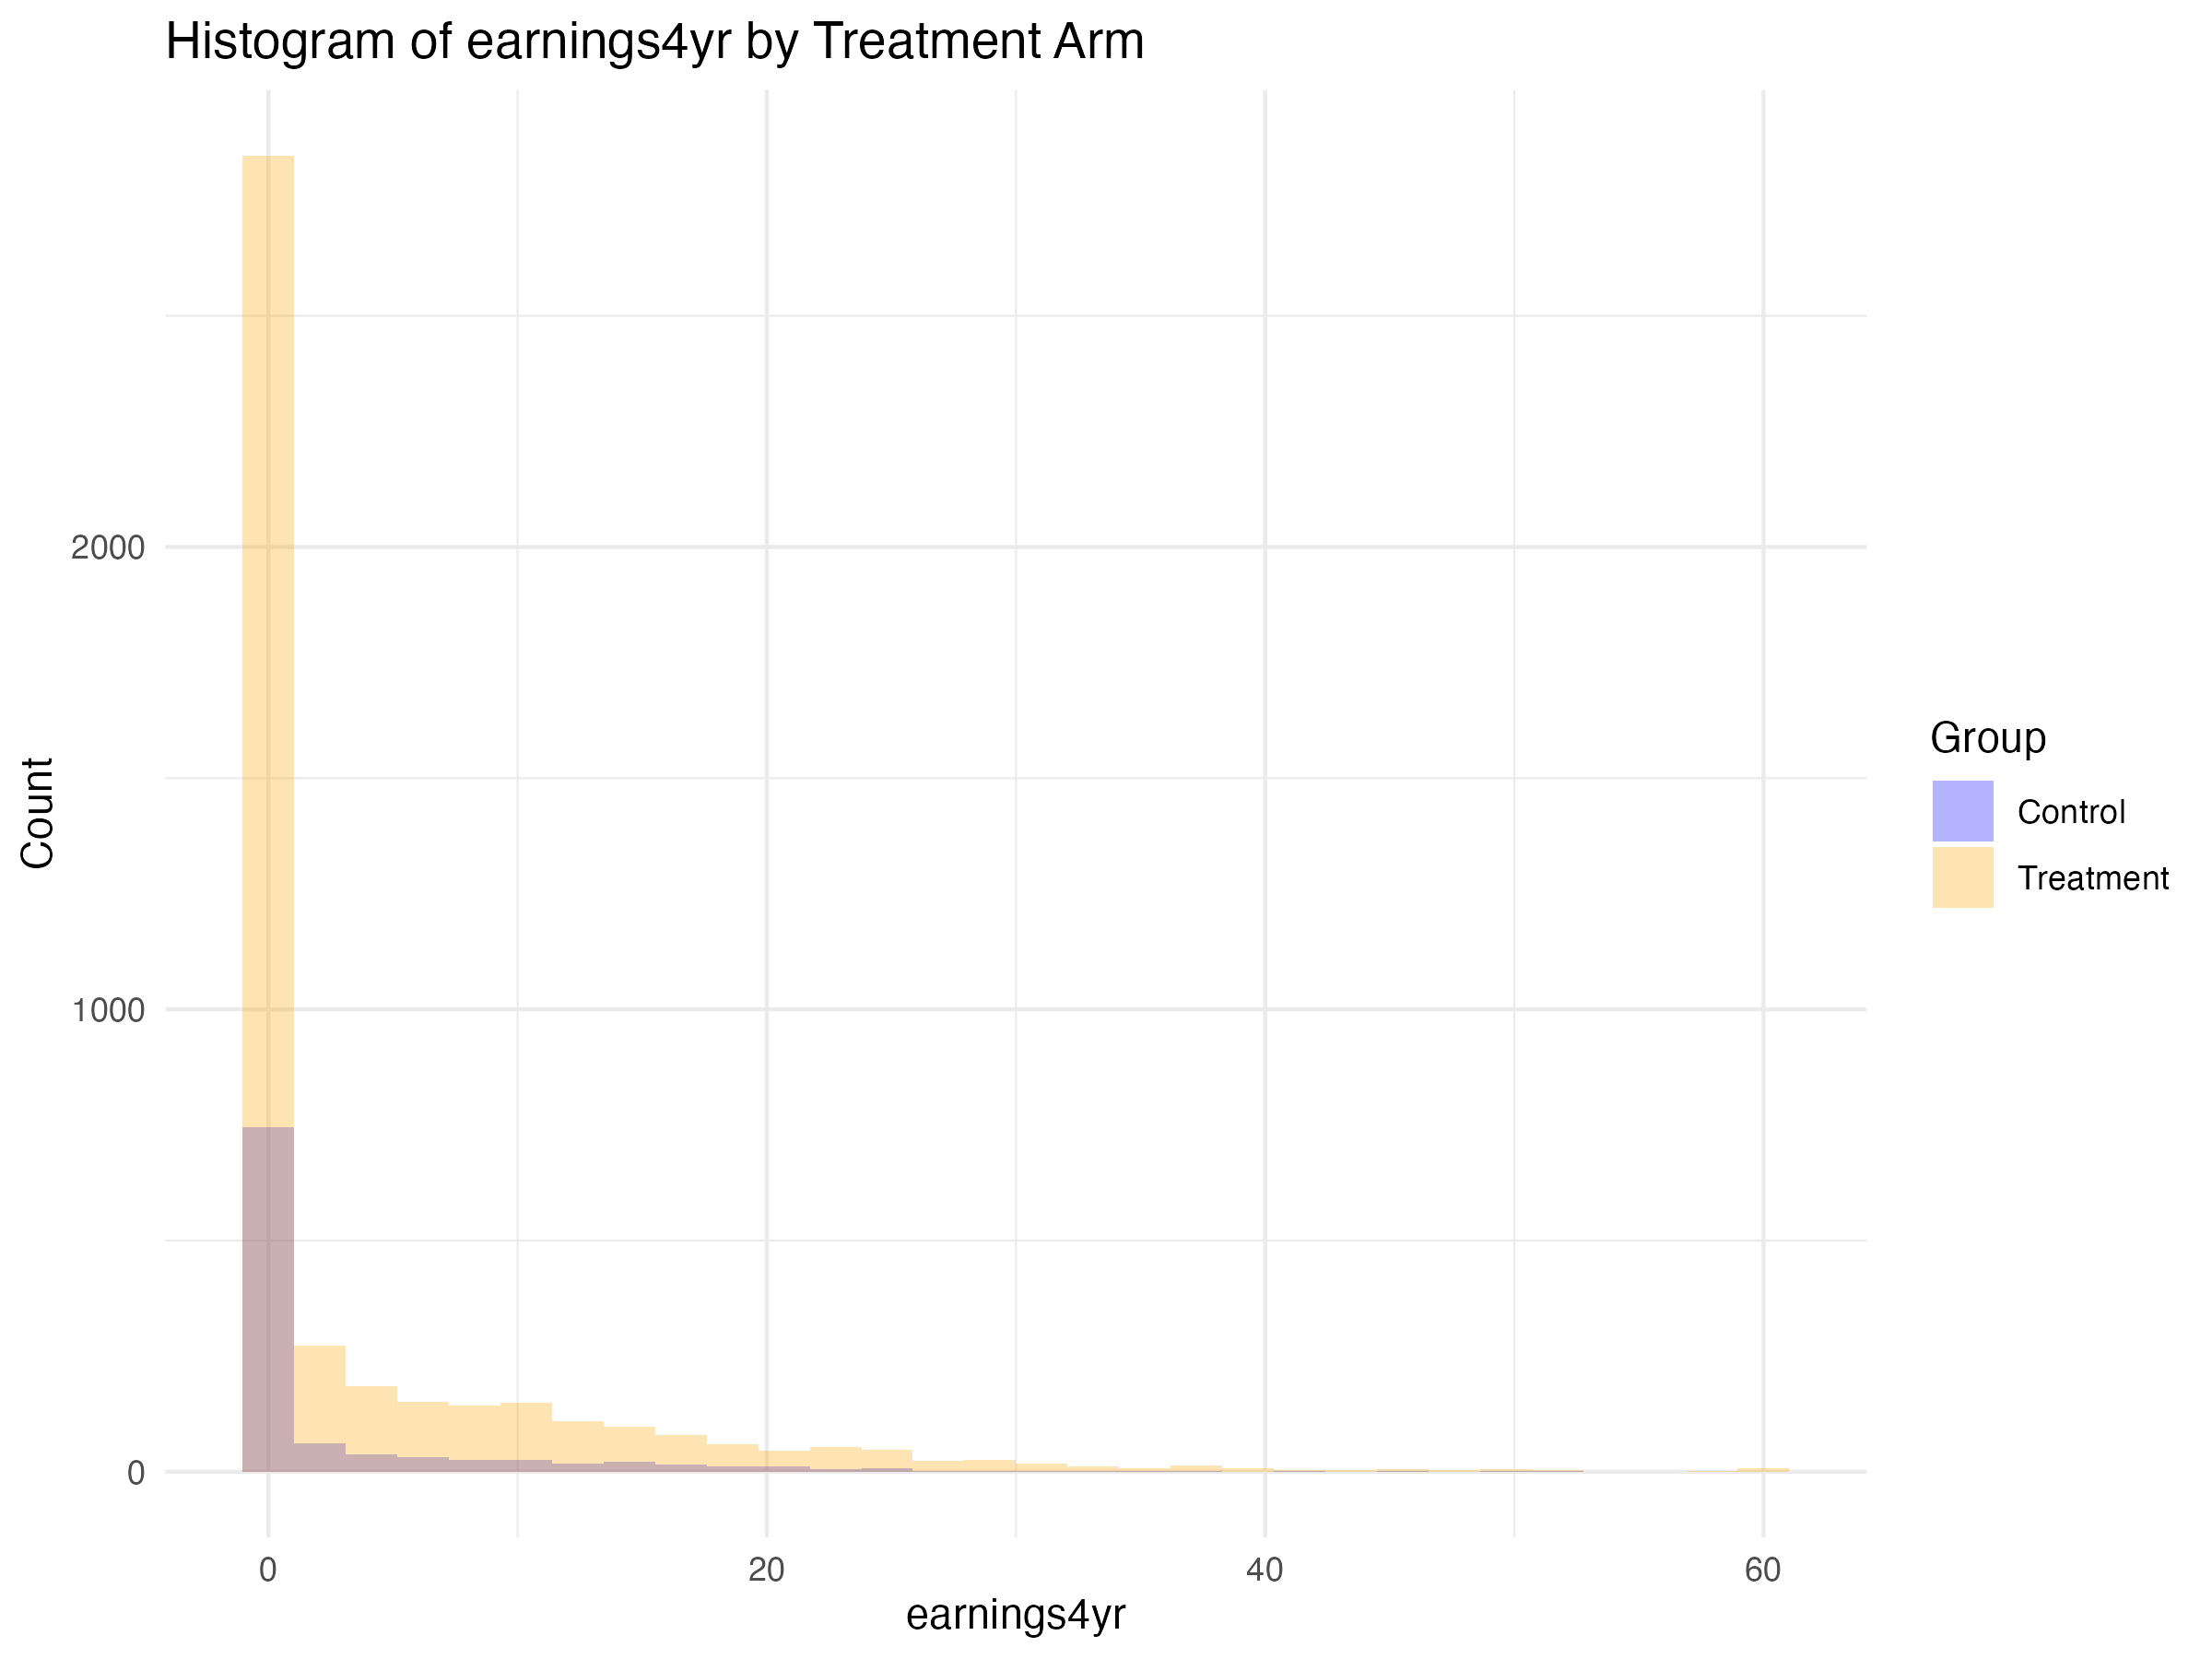
\includegraphics[width=0.8\textwidth]{output/histogram_earnings4yr_by_treatment_arm.png}
        \caption{\label{fig:hist_earnings4yr}Earnings four years after treatment}
    \end{subfigure}
    \caption{\label{fig:hist_earnings}Histograms of earnings one year and four years after treatment}
\end{figure}



\subsection*{(a) ATE estimation and 90\% confidence intervals}

For ATE estimation, I use the difference-in-means estimator with the following formula:

\begin{equation}
    \hat{\tau} = \frac{1}{N} \sum_{i=1}^N \bigl(W_iY_i - (1-W_i)Y_i\bigr)\label{eq:ATE_dim}
\end{equation}

where $W_i$ is the treatment indicator and $Y_i$ is the observed outcome.

For the Neyman variance estimator, I use the following formula:
\begin{equation}
    \hat{Var}(\hat{\tau}) = \frac{S_0^2}{N_0} + \frac{S_1^2}{N_1}\label{eq:neyman_var}
\end{equation}

where $S_0^2/N_0$ and $S_1^2/N_1$ are the sample variances divided by the sample sizes of the control and treatment groups, respectively.\footnote{Note that this estimates the first two terms of the actual Neyman variance where the potential outcomes are predetermined and the permutation of the treatment indicator is the source of randomness. The third term that considers the variance in the difference of the potential outcomes cannot be estimated here.}

\begin{align}
    \begin{cases}
    S_w^2 &= \frac{1}{N_w-1} \sum_{i=1}^N \bigl(\mathbb{I}\{W_i=w\}(Y_i - \bar{Y}_w)\bigr)^2\\
    \bar{Y}_w &= \frac{1}{N_w} \sum_{i=1}^N \bigl(\mathbb{I}\{W_i=w\}Y_i\bigr)
    \end{cases}
\end{align}

I use the following formula to estimate the 90\% confidence interval of the ATE:
\begin{equation}
    \hat{\tau} \pm 1.645 \sqrt{\hat{Var}(\hat{\tau})}\label{eq:ci}
\end{equation}

The results are shown in table \ref{tab: ATE_results}.

\begin{table}[h]
    \centering
    % latex table generated in R 4.5.1 by xtable 1.8-4 package
% Sat Oct  4 16:43:04 2025
\begin{tabular}{lrr}
  \hline
Statistic & earnings 1yr & earnings 4yr \\ 
  \hline
DIM estimate & 1.14 & 1.23 \\ 
  Neyman variance & 0.02 & 0.06 \\ 
  Homoskedastic variance & 0.03 & 0.08 \\ 
  Confidence interval lower bound & 0.92 & 0.82 \\ 
  Confidence interval upper bound & 1.36 & 1.64 \\ 
  Confidence interval lower bound (homoskedastic) & 0.86 & 0.77 \\ 
  Confidence interval upper bound (homoskedastic) & 1.42 & 1.69 \\ 
   \hline
\end{tabular}

    \caption{\label{tab: ATE_results}ATE results}
\end{table}



\subsection*{(b) Stratified ATE estimation}

I stratify the data into four groups based on high school degree and child status.
For each group, I estimate the ATE using the difference-in-means estimator and the Neyman variance estimator.
%The results are shown in table \ref{tab: stratified_ATE_results}.

That is, we have the following four groups:
\begin{itemize}
    \item High school degree and child: $TT$(0.096\%; 79\% are treated)
    \item High school degree and no child: $TF$(0.427\%; 81\% are treated)
    \item No high school degree and child: $FT$(0.068\%; 83\% are treated)
    \item No high school degree and no child: $FF$(0.4109\%; 80\% are treated)
\end{itemize}

For each group, I estimate the ATE using the difference-in-means estimator and the Neyman variance estimator following equations
\eqref{eq:ATE_dim} and \eqref{eq:neyman_var}.

The results are shown in tables \ref{tab: stratified_results_1yr} and \ref{tab: stratified_results_4yr} and figure \ref{fig:stratified_results}.

\begin{table}[h]
    \centering
    \small
    % latex table generated in R 4.5.1 by xtable 1.8-4 package
% Sat Oct  4 16:43:04 2025
\begin{tabular}{lrrrr}
  \hline
Group & DIM estimate & Neyman variance & Confidence interval lower bound & Confidence interval upper bound \\ 
  \hline
TT & 1.43 & 0.18 & 0.74 & 2.13 \\ 
  TF & 1.50 & 0.05 & 1.12 & 1.89 \\ 
  FT & 0.50 & 0.35 & -0.48 & 1.47 \\ 
  FF & 0.76 & 0.03 & 0.48 & 1.04 \\ 
   \hline
\end{tabular}

    \caption{\label{tab: stratified_results_1yr}Stratified ATE results (1yr)}
\end{table}

\begin{table}[h]
    \centering
    \small
    % latex table generated in R 4.5.1 by xtable 1.8-4 package
% Sat Oct  4 16:43:04 2025
\begin{tabular}{lrrrr}
  \hline
Group & DIM estimate & Neyman variance & Confidence interval lower bound & Confidence interval upper bound \\ 
  \hline
TT & 2.83 & 0.85 & 1.32 & 4.35 \\ 
  TF & 1.17 & 0.21 & 0.41 & 1.93 \\ 
  FT & 0.89 & 0.82 & -0.61 & 2.38 \\ 
  FF & 0.95 & 0.06 & 0.54 & 1.36 \\ 
   \hline
\end{tabular}

    \caption{\label{tab: stratified_results_4yr}Stratified ATE results (4yr)}
\end{table}

\begin{figure}[h]
    \centering
    \begin{subfigure}{0.48\textwidth}
    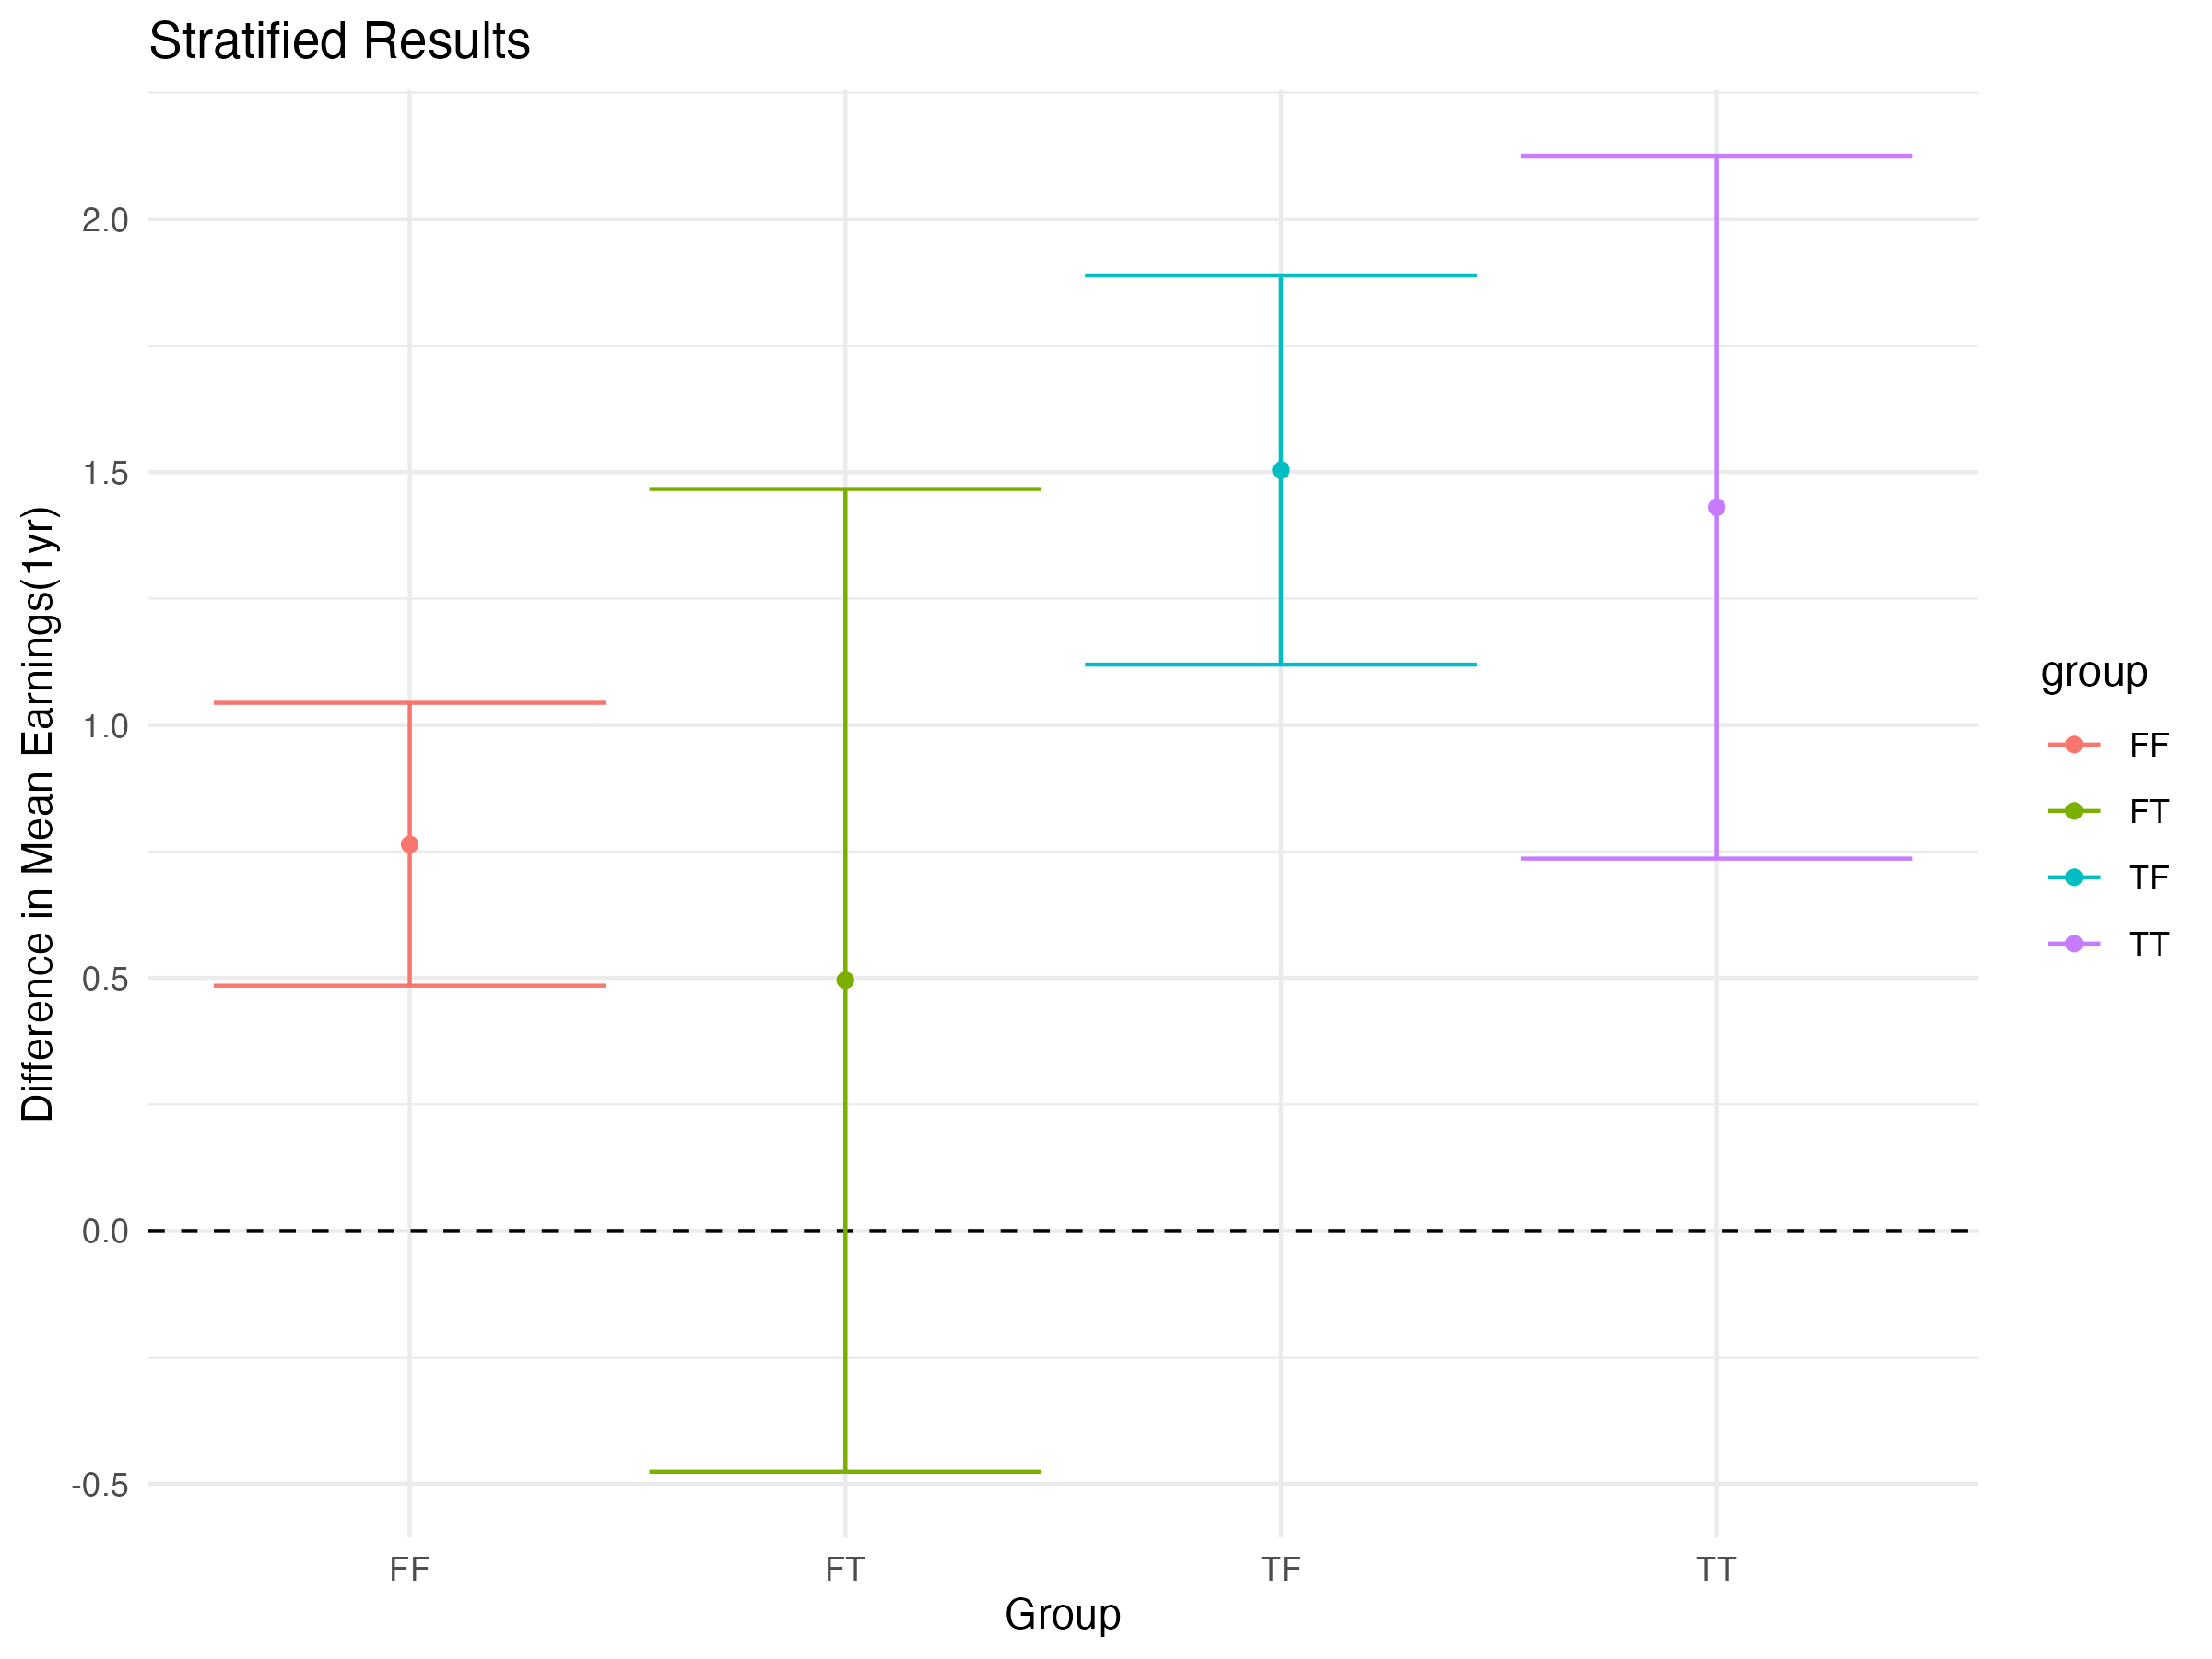
\includegraphics[width=\textwidth]{output/stratified_results_1yr.png}
    \caption{\label{fig:stratified_results_1yr}Earnings one year after treatment}
    \end{subfigure}
    \begin{subfigure}{0.48\textwidth}
    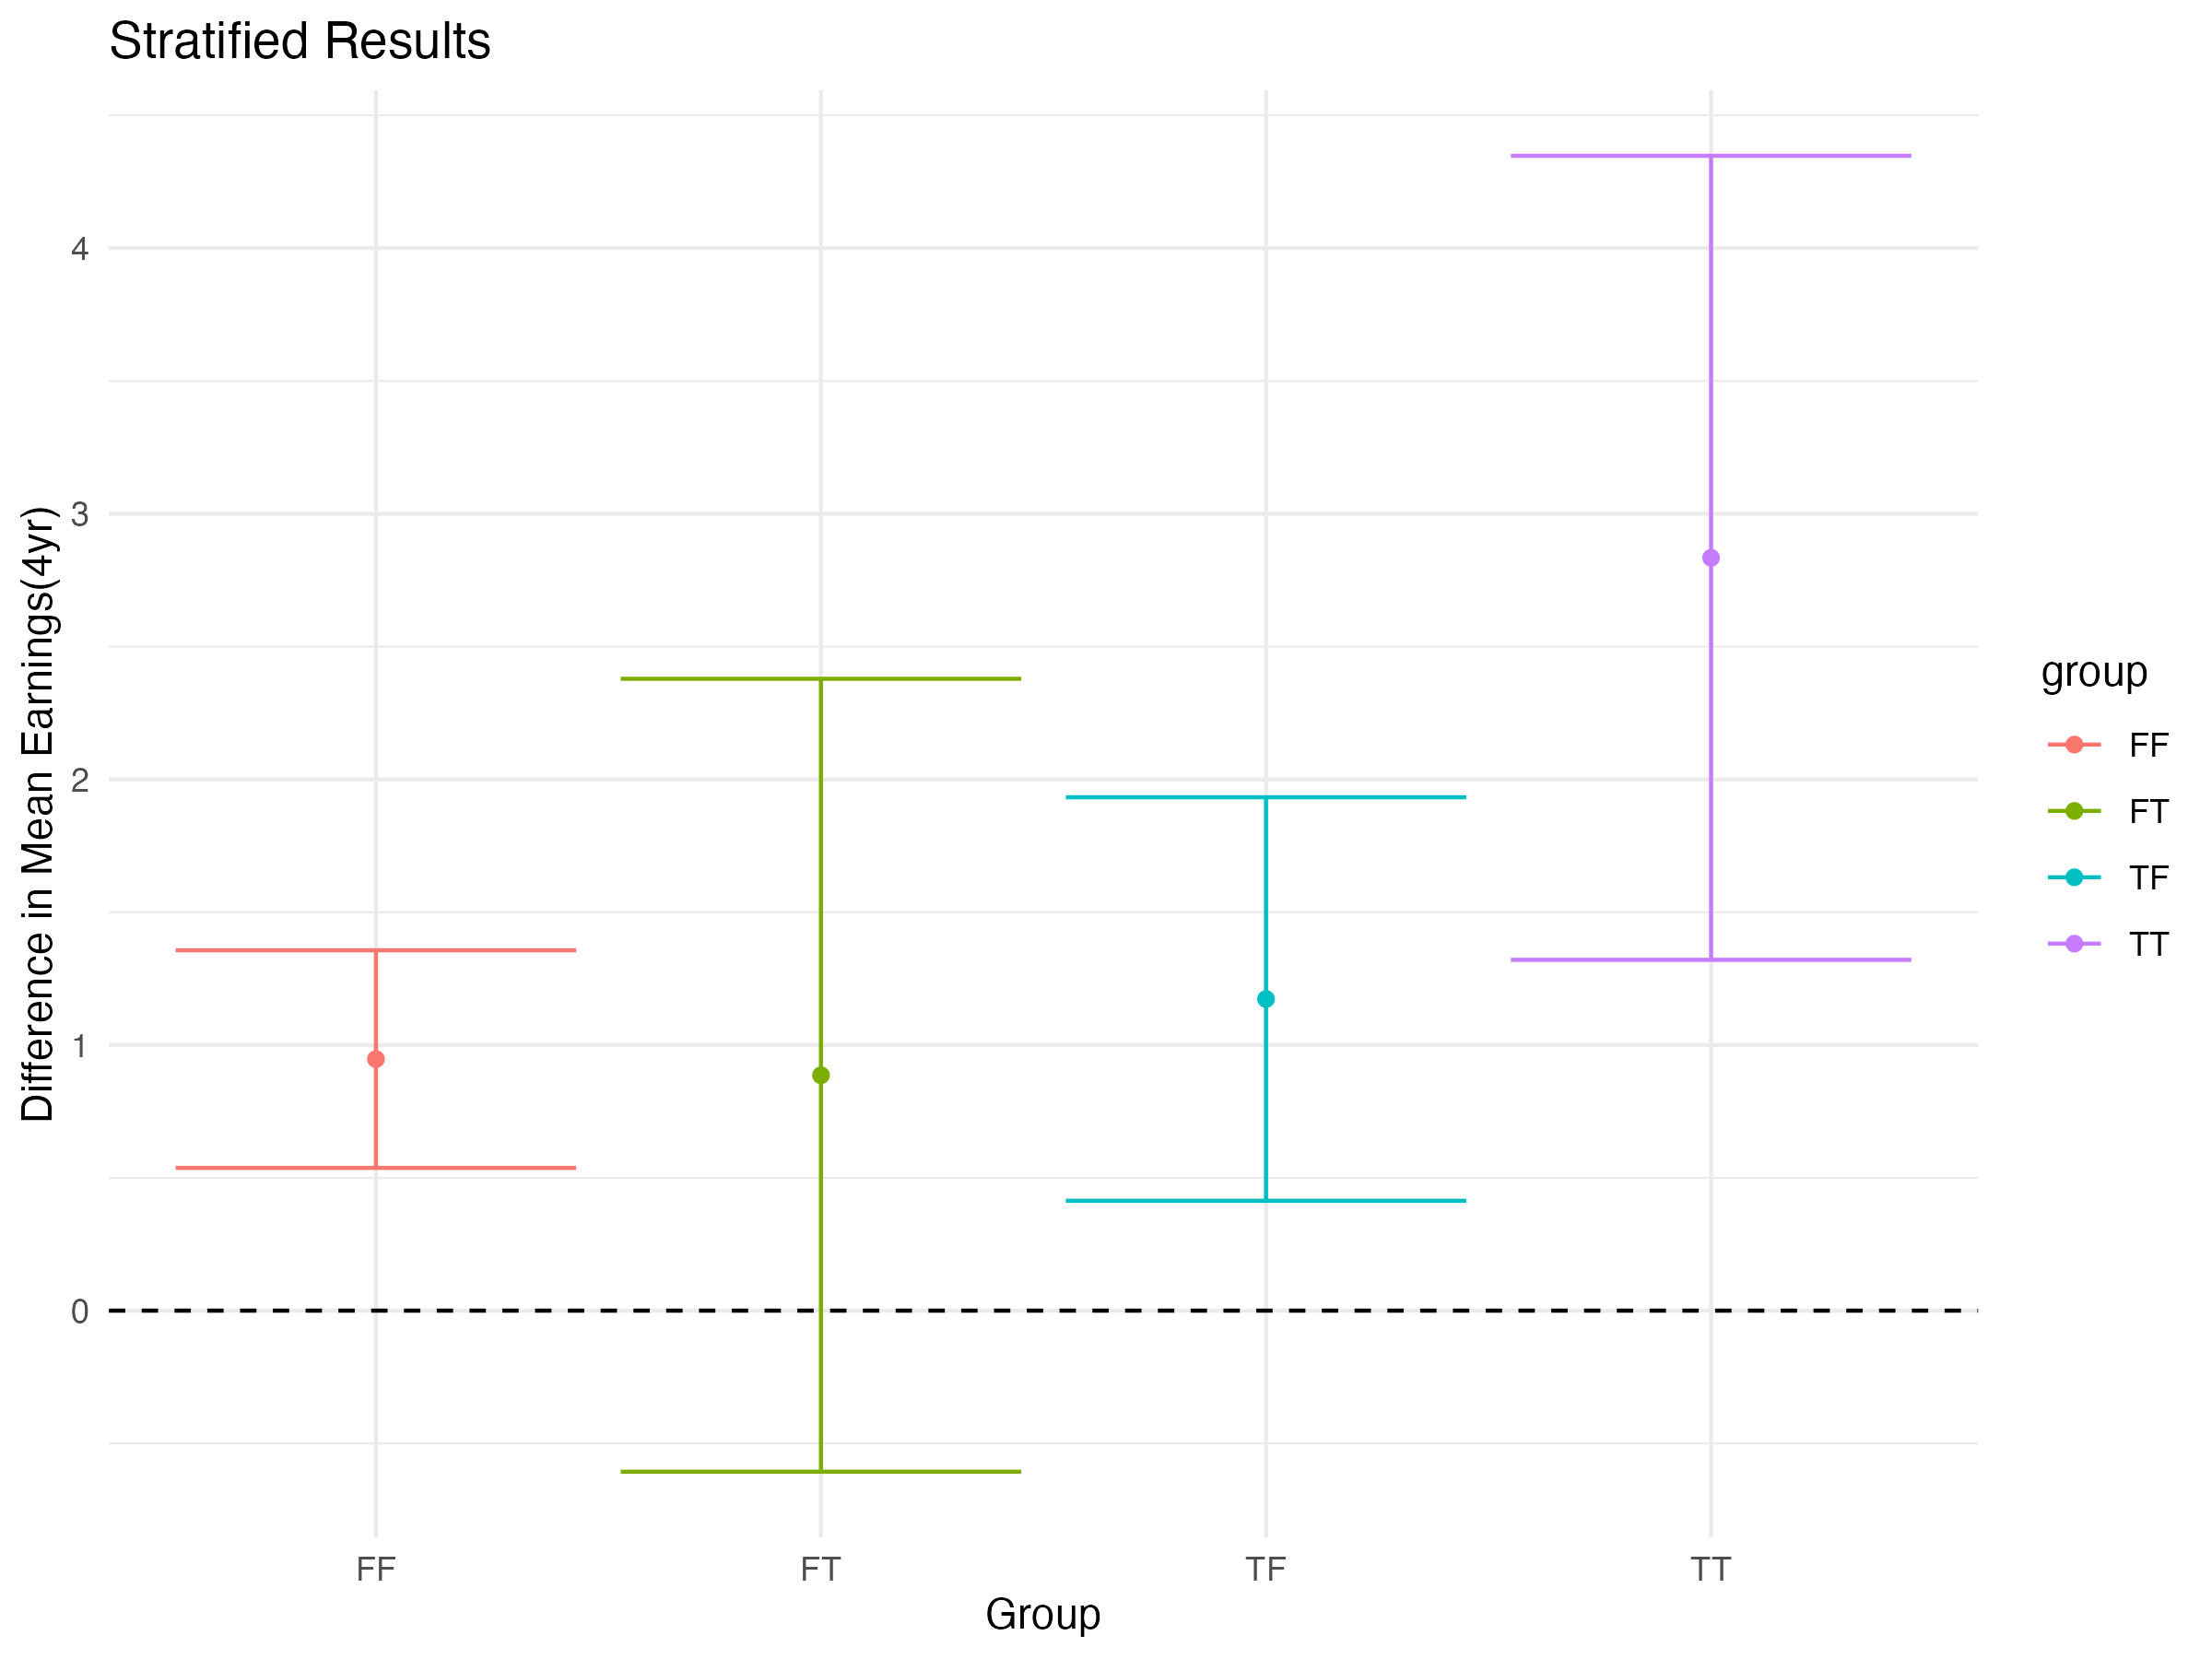
\includegraphics[width=\textwidth]{output/stratified_results_4yr.png}
    \caption{\label{fig:stratified_results_4yr}Earnings four years after treatment}
    \end{subfigure}
    \caption{\label{fig:stratified_results}Stratified ATE results (1yr and 4yr)}
\end{figure}



\subsection*{(c) Aggregation}

To obtain the aggregate ATE and the standard error, I use the following formula:
\begin{align}
    \hat{\tau} &= \sum_{g \in G} \frac{N_g}{N}\hat{\tau}_g \label{eq:aggregate_ATE}\\
    \hat{Var}(\hat{\tau}) &= \sum_{g \in G} \frac{N_g^2}{N^2}\hat{Var}(\hat{\tau}_g) \label{eq:aggregate_var}
\end{align}

where $G = \{TT, TF, FT, FF\}$ is the set of groups, $\hat{\tau}_g$ is the ATE for group $g$, and $N_g$ is the sample size of group $g$.\footnote{A critical assumption here is that the groups are independent of each other. Since the treatment assignment of an individual is correlated with the treatment assignment of others, this assumption is not satisfied in the Neyman world. However, I assume that the groups are independent of each other for the sake of simplicity.}
The results are shown in table \ref{tab: aggregate_results_1yr} and \ref{tab: aggregate_results_4yr}.

\begin{table}[h]
    \centering
    \small
    % latex table generated in R 4.5.1 by xtable 1.8-4 package
% Sat Oct  4 16:43:04 2025
\begin{tabular}{lr}
  \hline
Statistic & Value \\ 
  \hline
Aggregated DIM estimate & 1.13 \\ 
  Aggregated Neyman variance & 0.02 \\ 
  Aggregated CI lower bound (90\%) & 0.90 \\ 
  Aggregated CI upper bound (90\%) & 1.35 \\ 
   \hline
\end{tabular}

    \caption{\label{tab: aggregate_results_1yr}Aggregate ATE results (1yr)}
\end{table}

\begin{table}[h]
    \centering
    \small
    % latex table generated in R 4.5.1 by xtable 1.8-4 package
% Sat Oct  4 16:43:04 2025
\begin{tabular}{lr}
  \hline
Statistic & Value \\ 
  \hline
Aggregated DIM estimate & 1.22 \\ 
  Aggregated Neyman variance & 0.06 \\ 
  Aggregated CI lower bound (90\%) & 0.81 \\ 
  Aggregated CI upper bound (90\%) & 1.63 \\ 
   \hline
\end{tabular}

    \caption{\label{tab: aggregate_results_4yr}Aggregate ATE results (4yr)}
\end{table}


Comparing the estimates here to table \ref{tab: ATE_results} in section (a), we can see that the estimates and variances are pretty similar; however, the standard errors are based on different assumptions.
In the case of overall difference-in-means, the standard errors are based on the permutation of the treatment indicator, where the permutation is basically choosing 1,036 observations out of 5,419 observations to be treated.
This regards the number 1,036 as fixed.
On the other hand, in the case of stratified difference-in-means, the standard errors have a stronger assumption on the number of observations treated in each group.
That is, we are assuming the following numbers in table \ref{tab: balance} to be fixed.

\begin{table}[h]
    \centering
    % latex table generated in R 4.5.1 by xtable 1.8-4 package
% Sat Oct  4 17:00:38 2025
\begin{tabular}{lllr}
  \hline
Treatment & High School Degree & Child & Number of Obs. \\ 
  \hline
Control & No & No & 432 \\ 
  Treated & No & No & 1784 \\ 
  Control & No & Yes &  62 \\ 
  Treated & No & Yes & 306 \\ 
  Control & Yes & No & 433 \\ 
  Treated & Yes & No & 1883 \\ 
  Control & Yes & Yes & 109 \\ 
  Treated & Yes & Yes & 410 \\ 
   \hline
\end{tabular}

    \caption{\label{tab: balance}Number of observations in each subgroup}
\end{table}



\section{Part II}

For questions (a) and (b), I consider the following three random variables:

\begin{align}
    \hat\tau &= \frac{\sum_{i=1}^N W_iY_i}{\sum_{i=1}^N W_i} - \frac{\sum_{i=1}^N (1-W_i)Y_i}{\sum_{i=1}^N (1-W_i)} \label{eq:hat_tau}\\
    \tau_t &= \frac{\sum_{i=1}^N W_i\bigl(Y_i(1) - Y_i(0)\bigr)}{\sum_{i=1}^N W_i} \label{eq:tau_t}\\
    \tau_c &= \frac{\sum_{i=1}^N (1-W_i)\bigl(Y_i(1) - Y_i(0)\bigr)}{\sum_{i=1}^N (1-W_i)} \label{eq:tau_c}
\end{align}


\subsection*{Unbiasedness}

Then, I can show that $\mathbb{E}\bigl[\hat\tau - \tau_t\bigr] = \mathbb{E}\bigl[\hat\tau - \tau_c\bigr] =0$. 
In the following, note that $Y_i(1)$ and $Y_i(0)$ are considered constants.

\begin{align*}
    \mathbb{E}\bigl[\hat\tau - \tau_t\bigr] &= \mathbb{E}\biggl[\frac{\sum_{i=1}^N W_iY_i(1)}{N_1} - \frac{\sum_{i=1}^N (1-W_i)Y_i(0)}{N_0} - \frac{\sum_{i=1}^N W_i\bigl(Y_i(1) - Y_i(0)\bigr)}{N_1}\biggr]\\
    &= \mathbb{E} \biggl[\biggl(\frac{1}{N_1} + \frac{1}{N_0}\biggr)\sum_{i=1}^N W_iY_i(0) - \frac{1}{N_0}\sum_{i=1}^NY_i(0)\biggr]\\
    &= \biggl(\frac{1}{N_1} + \frac{1}{N_0}\biggr)\sum_{i=1}^N \mathbb{E} [W_i]Y_i(0) - \frac{1}{N_0}\sum_{i=1}^NY_i(0)\\
    &= \biggl(\frac{N}{N_0N_1}\biggr)\sum_{i=1}^N \frac{N_1}{N}Y_i(0) - \frac{1}{N_0}\sum_{i=1}^NY_i(0) = 0
\end{align*}

Sinilarly, we can show that $\mathbb{E}\bigl[\hat\tau - \tau_c\bigr] = 0$.

\subsection*{(a) and (b) - True Variances}

Here, I report the true variances of the following random variables: $\Var(\hat\tau - \tau_t)$ and $\Var(\hat\tau - \tau_c)$.\footnote{\color{blue}comment: I tried to derive the true variances of $\Var(\tau_t)$ and $\Var(\tau_c)$, but it turned out to be a function of the potential outcomes, which does not look feasible to me. Is it possible to derive them?}
Also, let us denote $\tau_i = Y_i(1) - Y_i(0)$, and it must be noted that every expectation and variances are conditional on 
$\sum_{i=1}^N W_i = N_1, \sum_{i=1}^N (1-W_i) = N_0, Y_i(1), \text{ and } Y_i(0)$.

\begin{align*}
    \Var_W(\hat\tau - \tau_t) &= \E_W((\hat\tau - \tau_t)^2) - \E_W^2[\hat\tau - \tau_t]\\
    &= \E_W((\hat\tau - \tau_t)^2) \\
    &=\mathbb{E}_W\biggl[ \biggl(\cancel{\frac{1}{N_1}\sum_{i=1}^N[W_iY_i]}-\frac{1}{N-N_1}\sum_{i=1}^N[(1-W_i)Y_i]- \frac{1}{N_1} \sum_{i=1}^N W_i[\cancel{Y_i(1)} - Y_i(0)]\biggr)^2\biggr]\\
     &= \mathbb{E}_W\biggl[ \biggl(-\frac{1}{N-N_1}\sum_{i=1}^N[(1-W_i)Y_i]+ \frac{1}{N_1} \sum_{i=1}^N W_i[Y_i(0)]\biggr)^2\biggr]\\
    &= \mathbb{E}_W\biggl[ \biggl(-\frac{1}{N-N_1}\sum_{i=1}^N[(1-W_i)Y_i(0)]+ \frac{1}{N_1} \sum_{i=1}^N W_i[Y_i(0)]\biggr)^2\biggr]\\
    &=\mathbb{E}_W\biggl[\biggl( \frac{N}{N_1(N-N_1)}\sum_{i=1}^NW_iY_i(0) - \frac{1}{N-N_1}\sum_{i=1}^N Y_i(0)\biggr)^2\biggr]\\
    &= \mathbb{V}_W\biggl( \frac{N}{N_1(N-N_1)}\sum_{i=1}^NW_iY_i(0) - \frac{1}{N-N_1}\sum_{i=1}^N Y_i(0)\biggr) \notag \\
    &+  \mathbb{E}_W^2 \biggl[\biggl( \frac{N}{N_1(N-N_1)}\sum_{i=1}^NW_iY_i(0) - \frac{1}{N-N_1}\sum_{i=1}^N Y_i(0)\biggr)\biggr]\\
    &= \mathbb{V}_W\biggl( \frac{N}{N_1(N-N_1)}\sum_{i=1}^NW_iY_i(0) - \frac{1}{N-N_1}\sum_{i=1}^N Y_i(0)\biggr) \notag \\
    &+ \underbrace{ \biggl( \frac{\cancel{N}}{\cancel{N_1}(N-N_1)}\sum_{i=1}^N\cancel{\mathbb{E}_W[W_i]}Y_i(0) - \frac{1}{N-N_1}\sum_{i=1}^N Y_i(0)\biggr)^2}_{=0}\\
    &= \biggl(\frac{N}{N_1(N-N_1)}\biggr)^2\mathbb{V}_W\biggl( \sum_{i=1}^NW_iY_i(0)\biggr)\\
    &= \biggl(\frac{N}{N_1(N-N_1)}\biggr)^2\biggl(\sum_{i=1}^NY_i(0)^2\underbrace{\frac{N_1}{N}(1-\frac{N_1}{N})}_{=\Var(W_i)} + \sum_{i=1}^N\sum_{j\neq i} Y_i(0)Y_j(0)\underbrace{\biggl(\frac{N_1(N_1-1)}{N(N-1)} - \frac{N_1^2}{N^2}\biggr)}_{\mathrm{Cov}(W_i, W_j)}\biggr)\\
    &= \biggl(\frac{1}{N_1(N-N_1)}\sum_{i=1}^NY_i(0)^2 - \frac{1}{N_1(N-1)(N-N_1)}\sum_{i=1}^N\sum_{j\neq i} Y_i(0)Y_j(0)\biggr)\\
    &= \frac{1}{N_1(N-N_1)}\sum_{i=1}^N Y_i(0)\biggl(\frac{N}{N-1}Y_i(0) - \frac{1}{(N-1)} \sum_{j=1}^N Y_j(0)\biggr)\\
    &= \frac{N}{N_1(N-N_1)(N-1)}\sum_{i=1}^N Y_i(0)\biggl(Y_i(0) - \bar{Y(0)} \biggr)\\
    &= \frac{N}{N_1(N-N_1)(N-1)}\biggl(\sum_{i=1}^N Y_i(0)^2 - \bar{Y(0)}^2 \biggr)\\
    &= \frac{N}{N_1N_0}S_1^2
\end{align*}


Likewise, we can show that $\Var_W(\hat\tau - \tau_c) = \frac{N}{N_1N_0}S_0^2$ by symmetry.

\subsection*{(a) and (b) - Unbiased Estimators for True Variances}

If we end up estimators $s_0^2$ and $s_1^2$ such that $\E(s_0^2) = S_0^2$ and $\E(s_1^2) = S_1^2$, respectively, we can obtain unbiased estimators for $\Var_W(\hat\tau - \tau_t)$ and $\Var_W(\hat\tau - \tau_c)$.

In this case of randomized experiment, we can use the following:

\begin{align}
    s_0^2 &= \frac{1}{N_0-1}\sum_{i=1}^N \bigl((1-W_i)(Y_i - \bar{Y}_0)\bigr)^2\label{eq:s_0^2}\\
    s_1^2 &= \frac{1}{N_1-1}\sum_{i=1}^N \bigl(W_i(Y_i - \bar{Y}_1)\bigr)^2\label{eq:s_1^2}
\end{align}

where $\bar{Y}_0$ and $\bar{Y}_1$ are the sample means of the control and treatment groups, respectively.


Therefore, the unbiased estimators for $\Var_W(\hat\tau - \tau_t)$ and $\Var_W(\hat\tau - \tau_c)$ are given by:

\begin{align}
    \hat{\Var}_W(\hat\tau - \tau_t) = \frac{N}{N_1N_0}s_1^2\label{eq:hat_var_tau_t}\\
    \hat{\Var}_W(\hat\tau - \tau_c) = \frac{N}{N_1N_0}s_0^2\label{eq:hat_var_tau_c}
\end{align}


\subsection*{(c) Variance of $\hat{\tau}$} 

The Neyman variance is given by:

\begin{equation}
    \Var_W(\hat\tau) = \frac{1}{N_1}S_1^2 + \frac{1}{N_0}S_0^2 - \frac{1}{N}S_{01}^2
\end{equation}

where $S_{01}^2 = \frac{1}{N-1}\sum_{i=1}^N \biggl(Y_i(1) - Y_i(0) - \tau \biggr)^2$.

The difficulty in the third term arises from the fact that either one of the two potential outcomes is not observed.
However, for the first two terms, we can use the unbiased estimators for $S_0^2$ and $S_1^2$ given by equations \eqref{eq:s_0^2} and \eqref{eq:s_1^2}.
Therefore, in cases where we have constant additive treatment effects, we can use the following unbiased estimator for $\Var_W(\hat\tau)$:

\begin{align}
    \hat{\Var}_W(\hat\tau) = \frac{1}{N_1}s_1^2 + \frac{1}{N_0}s_0^2  = \frac{N_1}{N}\hat{\Var}_W(\hat\tau - \tau_t) + \frac{N_0}{N}\hat{\Var}_W(\hat\tau - \tau_c)
\end{align}



%---- Appendix -----------------
\appendix
\setcounter{figure}{0}                      
\setcounter{table}{0}                      
\renewcommand\thefigure{A.\arabic{figure}} 
\renewcommand\thetable{A.\arabic{table}} 

\begin{sidewaystable}[h]
    \centering
    \tiny
    
\begin{tabular}{lrrrrrrrrrrrrrrrr}
\toprule
variable & numNA & numZeros & fracZeros & mean & sd & min & max & 10\% & 20\% & 30\% & 40\% & 50\% & 90\% & 95\% & 99\% & 99.9\%\\
\midrule
educ & 0 & 598 & 0.0018 & 12.7699 & 3.2812 & 0.0000 & 20.0000 & 9.0000 & 11.0000 & 12.0000 & 12.0000 & 12.0000 & 17.0000 & 19.0000 & 20.000 & 20.0000\\
lwage & 0 & 3 & 0.0000 & 5.8999 & 0.6788 & -2.3418 & 10.5321 & 5.2343 & 5.5218 & 5.7243 & 5.8472 & 5.9525 & 6.5567 & 6.8004 & 7.274 & 7.9495\\
yob & 0 & 0 & 0.0000 & 34.6028 & 2.9050 & 30.0000 & 39.0000 & 30.0000 & 32.0000 & 33.0000 & 34.0000 & 35.0000 & 39.0000 & 39.0000 & 39.000 & 39.0000\\
\bottomrule
\end{tabular}

    \caption{\label{tab:summary_stats}Summary Statistics}
\end{sidewaystable}


\begin{sidewaystable}[h]
    \centering
    \tiny
    
\begin{tabular}{lrrrrrrrrrrrrrrrr}
\toprule
variable & numNA & numZeros & fracZeros & mean & sd & min & max & 10\% & 20\% & 30\% & 40\% & 50\% & 90\% & 95\% & 99\% & 99.9\%\\
\midrule
W & 0 & 1,036 & 1.0000 & 0.0000 & 0.0000 & 0.0000 & 0.0000 & 0.0000 & 0.0000 & 0.0000 & 0.0000 & 0.0000 & 0.0000 & 0.0000 & 0.0000 & 0.0000\\
earnings1yr & 0 & 679 & 0.6554 & 1.4493 & 3.4950 & 0.0000 & 34.5994 & 0.0000 & 0.0000 & 0.0000 & 0.0000 & 0.0000 & 5.1112 & 8.6316 & 16.3443 & 28.6786\\
earnings4yr & 0 & 678 & 0.6544 & 3.0354 & 6.8941 & 0.0000 & 51.5277 & 0.0000 & 0.0000 & 0.0000 & 0.0000 & 0.0000 & 11.7650 & 17.7781 & 31.8940 & 51.4125\\
hs\_diploma & 0 & 494 & 0.4768 & 0.5232 & 0.4997 & 0.0000 & 1.0000 & 0.0000 & 0.0000 & 0.0000 & 0.0000 & 1.0000 & 1.0000 & 1.0000 & 1.0000 & 1.0000\\
female & 0 & 130 & 0.1255 & 0.8745 & 0.3314 & 0.0000 & 1.0000 & 0.0000 & 1.0000 & 1.0000 & 1.0000 & 1.0000 & 1.0000 & 1.0000 & 1.0000 & 1.0000\\
\addlinespace
age & 0 & 0 & 0.0000 & 33.8205 & 8.3839 & 15.0000 & 66.0000 & 25.0000 & 28.0000 & 29.0000 & 31.0000 & 33.0000 & 45.0000 & 49.0000 & 58.0000 & 62.9650\\
child & 0 & 865 & 0.8349 & 0.1651 & 0.3714 & 0.0000 & 1.0000 & 0.0000 & 0.0000 & 0.0000 & 0.0000 & 0.0000 & 1.0000 & 1.0000 & 1.0000 & 1.0000\\
single & 0 & 126 & 0.1216 & 0.8784 & 0.3270 & 0.0000 & 1.0000 & 0.0000 & 1.0000 & 1.0000 & 1.0000 & 1.0000 & 1.0000 & 1.0000 & 1.0000 & 1.0000\\
hs\_diploma\_dm & 0 & 0 & 0.0000 & 0.0000 & 0.4997 & -0.5232 & 0.4768 & -0.5232 & -0.5232 & -0.5232 & -0.5232 & 0.4768 & 0.4768 & 0.4768 & 0.4768 & 0.4768\\
female\_dm & 0 & 0 & 0.0000 & -0.0050 & 0.3314 & -0.8795 & 0.1205 & -0.8795 & 0.1205 & 0.1205 & 0.1205 & 0.1205 & 0.1205 & 0.1205 & 0.1205 & 0.1205\\
\addlinespace
age\_dm & 0 & 0 & 0.0000 & 0.1803 & 8.3839 & -18.6402 & 32.3598 & -8.6402 & -5.6402 & -4.6402 & -2.6402 & -0.6402 & 11.3598 & 15.3598 & 24.3598 & 29.3248\\
single\_dm & 0 & 0 & 0.0000 & 0.0125 & 0.3270 & -0.8658 & 0.1342 & -0.8658 & 0.1342 & 0.1342 & 0.1342 & 0.1342 & 0.1342 & 0.1342 & 0.1342 & 0.1342\\
\bottomrule
\end{tabular}

    \caption{\label{tab:summary_stats(control_group)}Summary Statistics}
\end{sidewaystable}


\begin{sidewaystable}[h]
    \centering
    \tiny
    
\begin{tabular}{lrrrrrrrrrrrrrrrr}
\toprule
variable & numNA & numZeros & fracZeros & mean & sd & min & max & 10\% & 20\% & 30\% & 40\% & 50\% & 90\% & 95\% & 99\% & 99.9\%\\
\midrule
W & 0 & 0 & 0.0000 & 1.0000 & 0.0000 & 1.0000 & 1.0000 & 1.0000 & 1.0000 & 1.0000 & 1.0000 & 1.0000 & 1.0000 & 1.0000 & 1.0000 & 1.0000\\
earnings1yr & 0 & 2,179 & 0.4971 & 2.5855 & 5.2141 & 0.0000 & 60.0000 & 0.0000 & 0.0000 & 0.0000 & 0.0000 & 0.0190 & 8.4014 & 11.7693 & 23.5991 & 56.8758\\
earnings4yr & 0 & 2,574 & 0.5873 & 4.2677 & 8.3822 & 0.0000 & 60.0000 & 0.0000 & 0.0000 & 0.0000 & 0.0000 & 0.0000 & 15.3113 & 22.4685 & 38.1191 & 60.0000\\
hs\_diploma & 0 & 2,090 & 0.4768 & 0.5232 & 0.4995 & 0.0000 & 1.0000 & 0.0000 & 0.0000 & 0.0000 & 0.0000 & 1.0000 & 1.0000 & 1.0000 & 1.0000 & 1.0000\\
female & 0 & 523 & 0.1193 & 0.8807 & 0.3242 & 0.0000 & 1.0000 & 0.0000 & 1.0000 & 1.0000 & 1.0000 & 1.0000 & 1.0000 & 1.0000 & 1.0000 & 1.0000\\
\addlinespace
age & 0 & 0 & 0.0000 & 33.5975 & 8.1511 & 16.0000 & 70.0000 & 24.0000 & 27.0000 & 29.0000 & 31.0000 & 33.0000 & 44.0000 & 49.0000 & 57.0000 & 61.6180\\
child & 0 & 3,667 & 0.8366 & 0.1634 & 0.3697 & 0.0000 & 1.0000 & 0.0000 & 0.0000 & 0.0000 & 0.0000 & 0.0000 & 1.0000 & 1.0000 & 1.0000 & 1.0000\\
single & 0 & 601 & 0.1371 & 0.8629 & 0.3440 & 0.0000 & 1.0000 & 0.0000 & 1.0000 & 1.0000 & 1.0000 & 1.0000 & 1.0000 & 1.0000 & 1.0000 & 1.0000\\
hs\_diploma\_dm & 0 & 0 & 0.0000 & 0.0000 & 0.4995 & -0.5232 & 0.4768 & -0.5232 & -0.5232 & -0.5232 & -0.5232 & 0.4768 & 0.4768 & 0.4768 & 0.4768 & 0.4768\\
female\_dm & 0 & 0 & 0.0000 & 0.0012 & 0.3242 & -0.8795 & 0.1205 & -0.8795 & 0.1205 & 0.1205 & 0.1205 & 0.1205 & 0.1205 & 0.1205 & 0.1205 & 0.1205\\
\addlinespace
age\_dm & 0 & 0 & 0.0000 & -0.0426 & 8.1511 & -17.6402 & 36.3598 & -9.6402 & -6.6402 & -4.6402 & -2.6402 & -0.6402 & 10.3598 & 15.3598 & 23.3598 & 27.9778\\
single\_dm & 0 & 0 & 0.0000 & -0.0030 & 0.3440 & -0.8658 & 0.1342 & -0.8658 & 0.1342 & 0.1342 & 0.1342 & 0.1342 & 0.1342 & 0.1342 & 0.1342 & 0.1342\\
\bottomrule
\end{tabular}

    \caption{\label{tab:summary_stats(treated_group)}Summary Statistics}
\end{sidewaystable}


\printbibliography

\end{document}